\documentclass{article}
\usepackage[french]{babel}
\usepackage{enumitem} 
\usepackage[utf8]{inputenc}
\usepackage{palatino}
\usepackage[T1]{fontenc}
\usepackage{fancyhdr}
\usepackage[french]{algorithm2e}
\usepackage{algpseudocode}
\usepackage{graphicx,float} % figure et placement de figure
\usepackage{listings} %%inclusion de programmes
\frenchbsetup{StandardLists=true}
\lstset{
language=C++,
basicstyle=\ttfamily\small, %
identifierstyle=\color{black}, %
keywordstyle=\color{blue}, %
stringstyle=\color{blue}, %
commentstyle=\it\color{green}, %
}

\usepackage{xcolor}

\pagestyle{fancy}
\lhead{\fontsize{10}{10}{M2IM - UCBL - 2014/2015}}
\chead{}
\rhead{Chemier \& Lhomme}

\lfoot{}
\cfoot{\thepage}
\rfoot{}

\title{Géométrie algorithmique et maillages \\
        Rapport projet de triangulation Delaunay}
\author{Aurélien Chemier 10908892 \\\texttt{aurelien.chemier71@gmail.com} \\
        Romane Lhomme 11006689  \\\texttt{romane.lhomme@gmail.com} }

\date{5 Janvier 2015}

\begin{document}

\maketitle
\tableofcontents
\newpage

\section{Introduction}
    L'objectif de ce projet, réalisé dans le cadre de l'unité d'enseignement \textit{"Géométrie algorithmique et maillages"} à l'Université Claude Bernard Lyon 1, était de générer la triangulation de Delaunay d'un terrain en $2D\frac{1}{2}$ à partir de points tirés aléatoirement en utilisant le principe du \textit{godness of fit} (ou affinage).
    \\La triangulation est produite à partir d'insertions itératives des points dans le maillage.
    
    \paragraph{}
    Le principe du \textit{godness of fit} consiste à insérer les points selon une priorité dépendant de la distance courante entre le maillage et le terrain. Ainsi, on insère en priorité les points les plus éloignés du maillage.
    
    \paragraph{}
    La triangulation de Delaunay consiste à vérifier, pour chaque triangle créé, que seuls les points présents dans le triangle circonscrit à ce triangle sont ceux qui le définissent. Lorsque l'on constate une anomalie, le maillage est modifié localement pour y remédier.
    
    \paragraph{}
    Afin de mener à bien ce projet, il nous a été demandé d'utiliser le language C pour implémenter les algortihmes et la bibliothèque graphique OpenGL afin d'avoir un aperçu des résultats. Nous avons également utilisé le gestionnaire de version Git afin de travailler facilement en collaboration.
    
\section{Utilisation du programme}
    Les paramètres par défaut d'utilisation du programme peuvent être modifiés via la ligne de commande.
    
    \begin{itemize}
    \item L'affichage du résultat dans une fenetre OpenGL doit être demandé avec l'argument $-a$ pour le squelette et $-t$ pour les triangles pleins et colorés.
    \item Le nombre de vertices est de 50 par défaut. Il peut être modifié avec l'argument $-n$ suivi du nombre de vertices voulu. 
    \\Exemple : $./delaunay -n100$
    \item Une triangulation naïve a également été implémentée. L'argument $-b$ permet de sélectionner cette triangulation. 
    \item Les différents critères d'arrêts pour la triangulation doivent être sélectionnés en ligne de commande:
        \begin{itemize}
        \item Le nombre de facettes à créer peut être modifié avec l'argument $-f$ suivi du nombre de facettes voulues. Par défaut toutes les facettes sont créés.
        \\Exemple : $./delaunay -f50$
        \item $-s$ modifie la valeur du seuil de distance minimale pour qu'un vertex puisse être inséré. Par défaut la distance minimale est à $0$. Ce seuil doit être exprimé sous forme pourcentage par rapport à la distance maximale et doit être compris dans l'intervale $[0;1[$.
        \\Exemple : $./delaunay -s0.2$ insérera les vertices donc la distance à la facette leur correspondant est supérieure à $20\%$ de la distance maximale possible.
        \end{itemize}
    \item L'aide peut être retrouvée avec l'argument $-h$.
    \end{itemize}
    
    Les différentes options peuvent être cumulées à l'exception de l'aide qui arrête le programme.
    
\section{Structures de base}
        Afin de pouvoir mettre en place un système de triangulation à partir de vertices, nous avons dû créer un certain nombre de structures de base.
        \\Si vous souhaitez avoir plus d'informations que celles données dans cette section, vous pouvez consulter la documentation Doxygen du projet.
    \subsection{Vertex}
    
        Le Vertex est la structure de base du projet, il permet de représenter les points qui formeront les sommets des simplexes.
    
    \begin{lstlisting}[caption={la structure Vertex},language=C,label=structvertex]
    typedef struct _Vertex
    {
        double coords[DIM]; 
        struct _Vertex *suivant;
    } Vertex;
    \end{lstlisting}
    
    \begin{itemize}
    \item \textit{coords} est le tableau des contenant les coordonnées du vertex. 
    Sa taille correspond au nombre de dimensions dans lequel le vertex est défini ; dans le cadre de ce projet \textit{DIM = 3}.
    \item \textit{suivant} est un pointeur sur un autre vertex. Il est utilisé pour la gestion des vertices dans la file de priorité de la structure \textit{Delaunay} (voir \ref{structureDelaunay}).
    \end{itemize}
    
    \subsection{Simplexe}
    
        La structure Simplexe permet de représenter les triangles.
     
    \begin{lstlisting}[caption={la structure Simplexe},language=C,label=structsimplexe]
    typedef struct _Simplexe
    {
        const Vertex *sommets[3];
        Vertex *listeVertex;
        Equation e;
        struct _Simplexe *voisins[3];
        double distanceMax;
        int indiceDansFile;
        struct _Simplexe *precedentPile;
        time_t marqueurTemps;
    } Simplexe;
    \end{lstlisting}
    
    \begin{itemize}
    \item \textit{sommets} contient les pointeurs sur les trois vertices qui composent le triangle. Ces trois sommets sont systématiquement ordonnés dans le tableau de manière à être définis dans le sens trigonométrique. Si tel n'était pas le cas, plusieurs fonctions et procédures n'auraient pas les résultats escomptés.
    \item \textit{listeVertex} est un pointeur sur le premier vertex de la liste des vertices qui appartiennent à ce simplexe mais n'ont pas encore été insérés. Le premier élément de cette liste est le vertex le plus éloigné du plan défini par le simplexe. On peut accéder aux autres éléments de la liste grâce à l'attribut \textit{suivant} de la structure \textit{Vertex}. Si il n'y a plus de vertex à insérer dans le simplexe, la liste pointe sur \textit{NULL}.
    \item \textit{e} contient les paramètres de l'équation définissant le plan formé par le simplexe. Elle est calculée à la création du simplexe et est de la forme suivante : \[a*x + b*y +c*z + d = 0\]
    \item \textit{voisins} contient les pointeurs sur les voisins du simplexe. Ils sont ordonnés de la manière suivante : le voisin en position $i$ correspond au simplexe géographiquement opposé au sommet $i$ ($i \in [0; \textit{DIM}-1]$).
    \item \textit{distanceMax} contient la distance entre le plan formé par le simplexe et le vertex le plus éloigné de ce plan. Si la liste de vertices est vide, la distance est de -1. Cette distance entre un vertex $v$ est le plan est calculée grâce à la formule suivante: \[| |-\frac{a * v.x + b*v.y + d}{c}| - |v.z| | \] avec 
    \begin{itemize}
    \item $a$, $b$, $c$ et $d$ les paramètres de l'équation du plan.
    \item $v.x$, $v.y$ et $v.z$ les coordonnés du vertex.
    \end{itemize}
    \item \textit{indiceDansFile} stocke comme son nom l'indique la position du simplexe dans la file de priorité (voir \ref{file}).
    \item Les éléments \textit{precedentPile} et \textit{marqueurTemps} sont utilisés dans le cas de la triangulation de Delaunay. Lorsque de nouveaux simplexes sont créés, ils sont ajoutés à la pile afin de pouvoir vérifier si il faut faire des échanges de diagonales. \textit{precedentPile} pointe sur le simplexe précédant dans la pile et \textit{marqueurTemps} permet d'indiquer si le simplexe a déjà été traité dans l'itération courante.
    \end{itemize}

    \subsection{File de Priorité}
    
    La file de priorité permet de trier les simplexes en fonction de leur attribut \textit{distanceMax}. Plus celle ci est élévée, plus le simplexe est prioritaire. Cette file de priorité est basée sur celle developpée en TP mais a été adaptée pour les simplexes.
    \\Elle se met à jour automatiquement à chaque ajout ou suppression d'élément ; une fonction est également disponible pour la mettre à jour lorsqu'un simplexe a été modifié (après un échange de diagonale par exemple).
    
    \begin{lstlisting}[caption={la structure FileSimplexe},language=C,label=structfile]
    typedef struct 
    {
       Simplexe ** file; 
       int nbElements;  
       int nbElementsCourant;
    } FileSimplexe;
    \end{lstlisting}
    \label{file}
    \begin{itemize}
    \item \textit{file} est un tableau de pointeurs sur des simplexes. Ce tableau est de taille $nbElements + 1$ car le premier élément d'une file de priorité se trouve à l'indice $1$.
    \item  \textit{nbElementsCourant} correspond au nombre de simplexes dans la file et donc au nombre de facettes créées.
    \end{itemize}

    \subsection{Delaunay}
    \label{structureDelaunay}
    
    Cette structure a été créée afin de regrouper les éléments nécessaires à la triangulation et de simplifier le passage des paramètres des fonctions et procédures.
    
    \begin{lstlisting}[caption={la structure Delaunay},language=C,label=structdelaunay]
        typedef struct 
        {
            FileSimplexe *filePrioriteSimplexe;
            Vertex *tableauVertex;
            int nbVertex;
            int nombreFacetteMax;
            double distanceMin;
        } Delaunay;
    \end{lstlisting}
    
    \begin{itemize}
    \item \textit{filePrioriteSimplexe} est un pointeur sur la file de priorité qui contient tous les simplexes.
    \item \textit{tableauVertex} est un tableau qui contient tous les vertices qui sont créés lors de l'initialisation puis qui seront associés à des simplexes. Ce tableau est de taille \textit{nbVertex}.
    \item \textit{nombreFacetteMax} et \textit{distanceMin} sont les variables qui permettent de gérer les cas d'arrêts de la triangulation (voir \ref{triangulationDelaunay}).
    \end{itemize}

\section{Initialisation}
    Avant de commencer la triangulation, une étape d'initialisation est nécessaire afin de tirer aléatoirement les coordonnées des vertices et de créer manuellement les deux premiers simplexes. Cette étape permet également d'initialiser la structure \textit{Delaunay}.
    
    \paragraph{}
    Le tableau de vertices est alloué en mémoire de manière à pouvoir contenir autant de vertices que le paramètre renseigné par l'utilisateur en ligne de commande. 
    Les quatres premiers vertices correspondent au quatres sommets du carré unitaire initial ($(0,0)$, $(1,0)$, $(1,1)$ et $(0,1)$). Les coordonnées en $x$, $y$ et $z$ de tous les autres vertices sont définis selon une loi aléatoire uniforme \[x,y \in[0;1[ ; z \in[0; \textit{H\_MAX}[\]
    
    \paragraph{}
    Il faut ensuite, à son tour, allouer la file de priorité. Par définition, le nombre maximum de simplexes pouvant être créés est égal à $2*(n - 1) - x$ avec:
        \begin{itemize}
        \item $n$ le nombre de vertices.
        \item $x$ le nombre de vertices composant l'enveloppe convexe.
        \end{itemize}
    Dans notre cas $x = 4$ ce qui nous donne au plus $2n - 6$ simplexes. Comme nous ne gérons pas de conteneur dynamique, on alloue autant de place que nécessaire pour stocker tous les simplexes dans la file de priorité.
    
    \paragraph{}
    Les quatres premiers vertices forment les deux premiers simplexes qui seront insérés dans la file : $((0,0), (1,0), (1,1))$ et $((0,0), (1,1), (0,1))$. Les voisins des simplexes sont initialisés à \textit{NULL} lorsque qu'il s'agit des bords du carré unitaire.
    \\Les vertices restants sont répartis dans les deux simplexes. Un vertex est à l'interieur d'un simplexe si sont projeté sur le plan $z=0$ est à l'intérieur du projeté du simplexe sur ce même plan.
    
    \paragraph{}
    Enfin, il faut initialiser les variables qui gérent les cas d'arrêt.
    \\Si aucune limite du nombre de facettes n'est passée en paramètre, la variable \textit{nombreFacetteMax} est alors égale à la taille maximum de la file de priorité. Sinon, c'est la valeur passée en paramètre qui sera stockée dans cette variable.
    \\La variable \textit{distanceMin} est initialisée à $0$ par défaut ; cela signifie que tous les vertices seront insérés car il n'y a pas de distance minimale à respecter. Si une valeur est passée en paramètre, elle est multipliée par \textit{H\_MAX} avant d'être stockée dans la structure.

    \paragraph{}
    \`{A} la fin de l'initialisation, tout est prêt pour que la triangulation se fasse de manière automatique.
    
\section{Triangulation}
    Pour la triangulation, nous avons procédé en deux étapes. Dans un premier temps, une triangulation naïve a été implémentée. La gestion des triangles avec l'algorithme de Delaunay n'a été mise en place que lorsque la première triangulation fonctionnait.
    
    \subsection{Cas d'arrêt}
    \label{triangulationDelaunay}
        La triangulation peut s'arrêter en fonction de deux paramètres qui sont passés par l'utilisateur. Ces deux paramètres ne sont pas mutuellement exclusifs. Si aucun paramètre n'est fourni, la triangulation s'arrête lorsque tous les vertices on été insérés.
        \\Voici les deux cas d'arrêt :
        \begin{itemize}
        \item On s'arrête si l'on atteint le nombre maximum de facettes demandé par l'utilisateur. 
        \\Etant donné qu'à chaque itération on crée trois simplexes et qu'on en supprime un, il est possible que le nombre final de facettes soit légèrement supérieur à celui renseigné par l'utilisateur.
        \item On s'arrête lorsque la valeur de l'attribut \textit{distanceMax} du simplexe en tête de la file de priorité est inférieure à la distance minimale demandée par l'utilisateur. Si cette distance est égale à $0$, tous les vertices seront insérés.
        \end{itemize}
    
    \paragraph{}
    Dans tous les cas, l'algorithme insère les vertices dans la triangulation tant qu'aucun des cas d'arrêt n'est satisfait.
        
    \subsection{Triangulation de base}
        \subsubsection{Algorithme}
           \label{algoBase}
             \begin{algorithm}[H]
             \SetKw{KwData}{Données}
             \SetKw{KwResult}{Résultats}
             \KwData{$fileS$ la file de priorité des simplexes contenant les deux simplexes initiaux}
             \newline
             \KwResult{$fileS$ la file contenant tous les simplexes créés}

             \While{(fileS.premier.distanceMax > distanceMin) \&\& (fileS.nbElementsCourant > nbFacetteMax)}{
              simplexe = premierFile\;
              vertex = simplexe.vertexLePlusLoin\;
              listeVertexTemp = vertex.suivant\;
              
              s1, s2, s3 = nouveaux simplexes à partir de $simplexe$ et $vertex$
              \ForEach{$s$ in \{s1, s2, s3\}}
              {ajoutDesVoisins(s)\;}
              \ForEach{$voisin$ in simplexe.voisins}
              {changementDeVoisin(voisin, simplexe, nouveauVoisin)\;}
              \ForEach{$v$ in listeVertexTemp}
              {repartitionDansLesNouveauxSimplexes(v)\;}
              ajoutDansLaFile(s1)\;
              ajoutDansLaFile(s2)\;
              ajoutDansLaFille(s3)\;
              suppression(simplexe)\;
             }
             \caption{Algorithme de triangulation naïve}
            \end{algorithm}
            
        \paragraph{}
        Lors de la création de chaque simplexe dans cet algorithme, les sommets sont rangés dans l'ordre trigonométrique pour garantir le bon fonctionnement du programme et une certaine simplicité de raisonnement.
            
        \subsubsection{Efficacité}
        
        Voici, pour un nombre de vertices données, le temps, en secondes, d'exécution de la triangulation (l'affichage n'est pas pris en compte). Les tests ont été effectués sur l'une de nos machines personnelles et peuvent varier d'un ordinateur à un autre.
       
        \begin{center}
            \begin{tabular}{|c|c|}\hline \label{tempsBasique}
                Nombre de vertices & Temps d'exécution (s) \\
                \hline
                $10$ & 0.005338 \\
                $100$ & 0.005810 \\
                $1000$ & 0.007804 \\
                $10^4$ & 0.032356 \\
                $10^5$ & 0.267649 \\
                $10^6$ & 3.078548 \\
                $10^7$ & 41.693276 \\
                \hline
            \end{tabular}
        \end{center}
        
        
        L'augmentation de la durée reste globalement linéaire ($o(N)$) ; seule la gestion de la file de priorité s'effectue en $o(\log{n})$.

    \subsection{Triangulation de Delaunay}
        \subsubsection{Algorithme}
        
        La triangulation de Delaunay consiste à ajouter à l'algorithme naïf (voir \ref{algoBase}) une boucle qui va contrôler, pour chaque simplexe, qu'il n'y a pas de vertices autres que les sommets de ce simplexe dans son cercle circonscrit.
        \\Après l'ajout des nouveaux simplexes créés dans la file, on les insère également dans la pile qui sera gérée par la boucle suivante.
        
        \paragraph{}
        \begin{algorithm}[H]
            \label{algoDelaunay}
            \SetKw{KwData}{Données}
            \KwData{p Une pile de Simplexe} \\
            \While{p non vide}{
                simplexe = sommetPile(p)\;
                \ForEach{voisin de simplexe}
                    {SommetOppose = sommet de voisin qui n'est pas dans simplexe\;
                    \If{SommetOppose appartient à Cercle de Simplexe} {
                       echangeSimplexe(simplexe, voisin)\;
                       retriFile(Simplexe)\;
                       retriFile(voisin)\;
                       ajoutPile(simplexe)\;
                       ajoutPile(voisin)\;}}}
            \caption{Boucle supplémentaire pour la triangulation de Delaunay}
       \end{algorithm}
       
       \subsubsection{Echange de diagonale}
       \label{echangeDiagonale}
        La fonction \textit{echangeSimplexe} qui peut aussi être appellée \textit{swap} consiste à changer la diagonale commune de deux simplexes afin que la condition de Delaunay soit respectée. Ainsi deux simplexes ABC et et ACD deviendront ABD et BCD (voir figure \ref{fig1}).
        
        \begin{figure}[H]
            \centering
            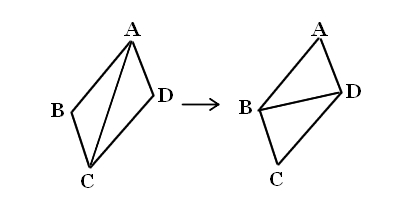
\includegraphics[scale=0.40]{exemple_swap_simple.jpg}     
            \caption{Echange de diagonale}
            \label{fig1}
        \end{figure}
        
        Nous avons essayé de faire un échange de diagonale le plus générique possible afin d'avoir une méthode claire et précise. Par la suite, nous supposerons que les deux simplexes dont nous voulons changer la diagonale se nomment S1 et S2.
        \\ Dans un premier temps, nous cherchons à connaître l'indice du sommet de S1 opposé à S2 ainsi que celui du sommet de S2 opposé à S1, que nous appellerons respectivement iS1 et iS2. Nous avons donc la configuration suivante : 
        
        \begin{figure}[H]
            \centering
            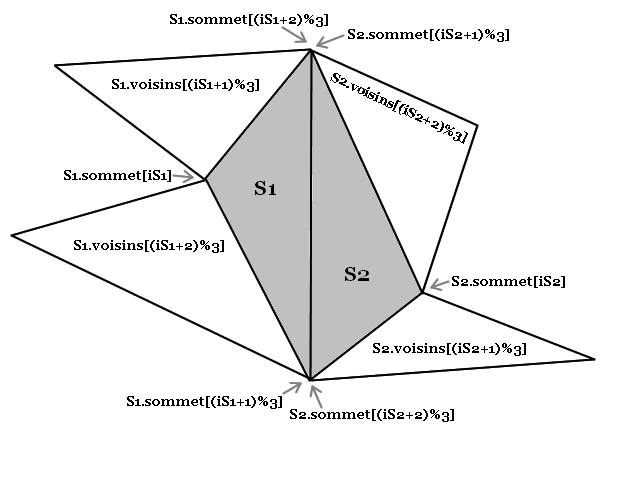
\includegraphics[scale=0.40]{config_avant_swap.jpg}     
            \caption{Configuration avant l'échange}
        \end{figure}
        
        Grâce à cette configuration, il nous est possible de créer les nouveaux simplexes aisément, quel que soit l'indice du sommet opposé à S2. Les vertices composant les sommet de S1 sont stockés dans un tableau temporaire ; de même pour les voisins de S1 et les voisins de S2. On stocke également le sommet de S2 opposé à S1.
        \\Tous ces éléments nous permettent de créer les deux nouveaux simplexes en changeant dans les structures de données des simplexes d'origine les valeurs qui correspondent à la configuration suivante :
        
        \begin{figure}[H]
            \centering
            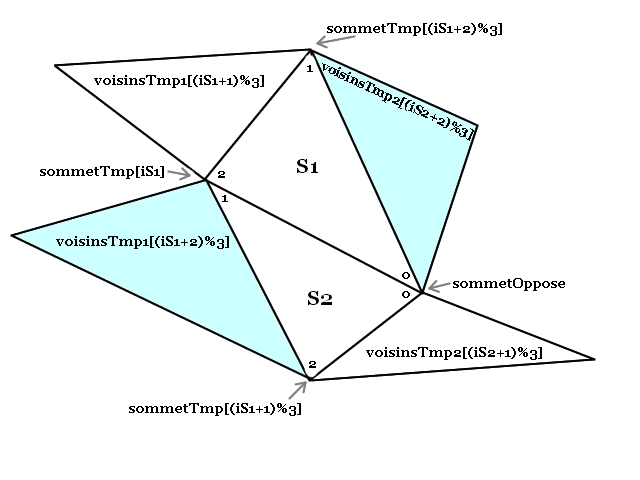
\includegraphics[scale=0.40]{config_apres_swap.jpg}     
            \caption{Configuration après l'échange}
            \label{fig3}
        \end{figure}
        
        Une fois que la diagonale a été changée, nous stockons les listes des vertices restants à insérer dans un temporaire puis nous les distribuons dans les deux nouveaux simplexes. 
        \\Il faut enfin notifier les deux voisins de S1 et S2 concernés (en bleu sur la figure \ref{fig3}) qu'ils ont changé de voisin.
        
        \subsubsection{Efficacité}
        
        Voici, pour un nombre de vertices données, le temps, en secondes, d'exécution de la triangulation avec l'échange de diagonale si nécessaire (l'affichage n'est pas pris en compte). Les tests ont été effectués sur l'une de nos machines personnelles et peuvent varier d'un ordinateur à un autre.
        
        \begin{center}
            \begin{tabular}{|c|c|}\hline \label{tempsDelaunay}
                Nombre de vertices & Temps d'exécution (s) \\
                \hline
                $10$ &  0.005565 \\
                $100$ & 0.005951 \\
                $1000$ & 0.011019 \\
                $10^4$ & 0.062287 \\
                $10^5$ & 0.536949 \\
                $10^6$ & 6.881539 \\
                $10^7$ & 85.979735 \\
                \hline
            \end{tabular}
        \end{center}
        
        L'ajout de cette boucle augmente la complexité de l'algorithme car il n'est pas possible de savoir à l'avance la taille maximale que va atteindre la pile et le nombre de fois que la fonction d'échange de diagonale va être appelée. C'est cette dernière qui augmente la compléxité de l'algorithme et allonge le temps d'exécution du programme car elle nécessite de replacer dans la file de priorité les simplexes qui ont été modifiés. 
        \paragraph{}
        D'après les résultats que nous avons obtenu, nous pouvons affirmer que le programme s'exécute en temps logarithmique, comme nous pouvions espérer.


\section{Conclusion}    

    L'objectif principal de ce projet, à savoir la triangulation d'un terrain en utilisant le principe de Delaunay et du \textit{godness of fit} a été atteint. En effet, nos simplexes sont correctement créés et l'on peut voir que l'échange de diagonale fonctionne lorsque l'on affiche le résultat dans une fenêtre OpenGL. Nous avons également fourni une méthode de triangulation naïve qui utilise uniquement le principe de \textit{godness of fit}.
    
    \paragraph{}
    La plus grande difficulté que nous avons rencontré a été l'implémentation de la fonction d'échange de diagonale et nous avons du procéder par étapes afin d'obtenir le résultat escompté. Dans un premier temps, nous avons traité les configurations initiales des simplexes cas par cas en fonction de leur orientation. Une fois que cette méthode fonctionnait, nous sommes passés à une implémentation plus générique (voir \ref{echangeDiagonale}).

\end{document}
